\section{Results}

We investigate the effect or near versus far fixation on eye-movement driven self-motion perception. Participants were presented with two subsequent translation movements (Figure 1) and had to judge whether the second was longer or shorter than the first. During each interval, participants fixated either a body- or world-fixed fixation point either nearby (50 cm) or far away (200 cm) from the participant.

%[While I realize that we switched the order of figure 2/3 in paper 3, I think it is better to retain the original order for paper 4].

\begin{figure}
    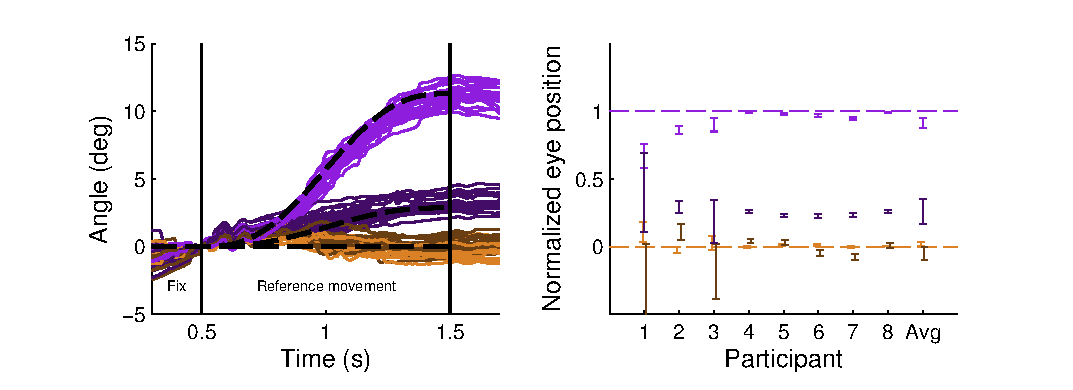
\includegraphics[width=1.0\textwidth]{src/paper4/paper4_figure2.eps}

    \caption{A. Actual (solid lines) and ideal (dashed lines) eye movement traces of one participant in the body-fixed (brown and orange) and world-fixed conditions (purple and pink). Gaze was directed at a near (brown and purple) or far (orange and pink) target. All traces shown are for 10m reference movements. B. [Need to decide what to put here.]}
    \label{p4:fig2}
\end{figure}

We first tested the ability of participants to follow eye movement each of the four main conditions (see \tabref{p4:tab1}). Exemplar eye traces for the 10cm reference translation each main condition are depicted in \figref{p4:fig2}A. As expected, eye movements are largely absent in the body near and body far conditions (brown and orange respectively). Following simple geometry, the eye movements were large when fixating nearby targets (purple) and small when fixating far away ones (pink). A similar pattern emerges when looking at the average normalized eye displacement (see Methods) for all participants (\figref{p4:fig2}B).  The normalized eye angle is about zero in body fixed fixations (brown and orange) and follows geometry in the world fixed fixations (purple and pink).  

%[NOTE: It seems quite difficult to say something about the vergence angle; our main point concerns the different version angle between world near/far.]

\begin{figure}
    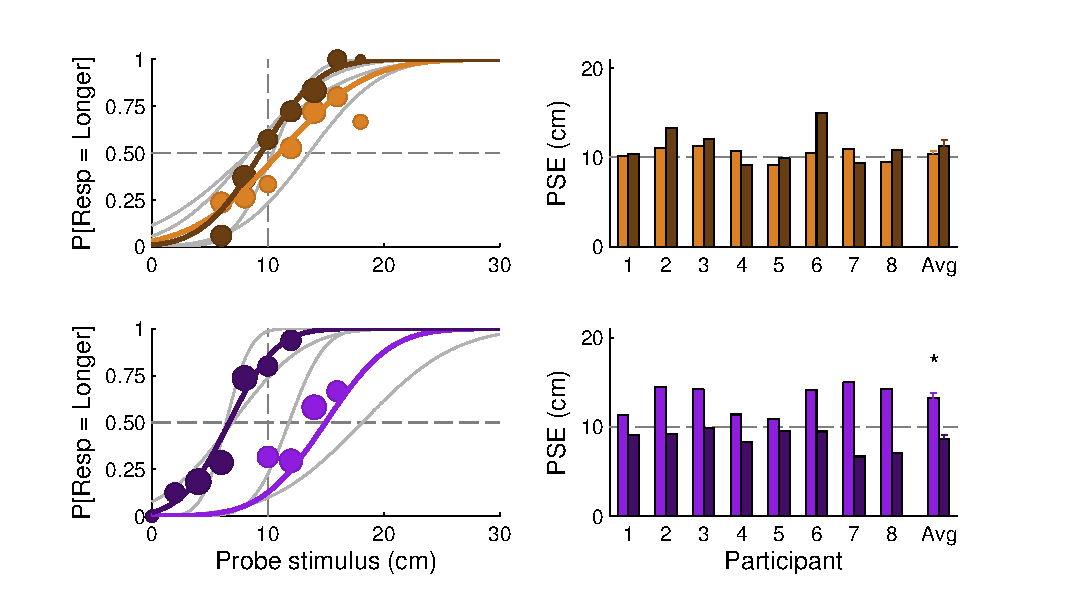
\includegraphics[width=1.0\textwidth]{src/paper4/paper4_figure3.eps}

	\caption{Psychometric curves (colored lines) and associated binned data (circles) for one participant. Circle size represents the amount of trials within the bin. Psychometric curves before collapsing across reference order are shown as gray lines. A.  Body-fixed condition while fixation was either near (brown) or far (orange). B. World-fixed condition while fixation was either near (purple) or far (pink).}
	\label{p4:fig3}
\end{figure}


The performance of a one participant is illustrated in the left column of Figure 3. Each rows shows one main condition: body near versus body far (Figure 3A; brown and orange), and world near versus world far (\figref{p4:fig3}B; purple and pink). The ligher and darker colors indicate which fixation type was the reference movement (see Legend). The shift of the psychometric functions relative to the 10 \si{\centi\metre} reference (i.e. the PSE) quantifies the influence of fixation distance. For example, the rightward shift of the pink curve in Figure 3B means that for a far world fixation a longer translation (~15cm) was required for that translation to be perceived equivalent to a 10 \si{\centi\metre} reference translation with world near fixation. On the other hand, the leftward shift of the purple curve means that a shorter translation with world near fixation (~6cm) was requird for that translation to be perceived equivalent to the 10cm reference translation with world far fixation. Together, these oppositely directed shifts demonstrate that translations with world far fixation were perceived shorter than equivalent translations with world near fixation. The brown and orange curves in \figref{p4:fig3}A do not show such shift, indicating that fixation depth (i.e. near versus far) has no effect in absense of eye movements (i.e. when fixating a body fixed target).

Similar results were obtained for all participants, as shown by the individual PSEs (right column of \figref{p4:fig3}). Statistical significance of the effects of fixation depth was evaluated by comparing PSEs between the two reference conditions using a paired t-test. The PSEs were significatly different in case of world-fixed fixations, t(7) = 5..42; p < 0.01 (\figref{p4:fig3}C), no such systematic difference was found for body-fixed fixations however, t(7) = -1.17; p = 0.28 (\figref{p4:fig3}D). As in the example subject, these results indicate that fixation depth does not influence self-motion perception during body fixed fixations. Fixating further away causes self-motion to be perceived as shorted in the world-fixed fixation condition however.

\begin{table}
    \begin{tabular}{l|lll}
	Participant & $\alpha_{50}$ & $\alpha_{200}$ & $\alpha$ \\
    \hline
	1 & 0.37 & 0.25 & 0.27 \\
	2 & 0.51 & 0.41 & 0.27 \\
	3 & 0.36 & 0.30 & 0.35 \\
	4 & 0.14 & 0.29 & 0.06 \\
	5 & 0.11 & 0.04 & 0.13 \\
	6 & 0.49 & 0.15 & 0.33 \\
	7 & 0.40 & 0.53 & 0.58 \\
	8 & 0.42 & 0.35 & 0.21 \\
    \end{tabular}

    \caption{.}

    \label{p4:tab2}
\end{table}

\begin{figure}
    \includegraphics[width=0.5\textwidth]{src/paper4/paper4_figure4.eps}

	\caption{PSEs for all participants and the average \textpm SE. A.  Body-fixed condition while fixation was either near (brown) or far (orange). B. World-fixed condition while fixation was either near (purple) or far (pink).}
	\label{p4:fig4}
\end{figure}

In order to quantify how much of the fixation depth was compensated for, we first created a simple linear model (see Methods) which attempts to explain perceived translation distance as a weighted average of a vestibular estimate (equal to the actual translation) and an oculomotor estimate (equal to the normalized eye movement times the actual translation; Equation 2).  The weighting parameter was depth dependent allowing it to compensate for fixation depth. As we used only two depths, this resulted in one weighting parameter per depth,  and  (see Table 2 for values). The predicted PSEs are plotted against the actually observed and PSEs in Figure 4. The positive correlation (ρ = 0.xx, p < 0.01) between observed and predicted PSEs shows that our simple models does reasonably well in predicting perceptual performance.

As the weighing parameters encompassed both depth dependent as well as depth independent effects, it is possible to remove the depth independent effects by taking the ratio between the two parameters. The ratio between  and  is plotted per participant in Figure 5. In case there is no depth compensation, i.e. when , the expected ratio is one. Perfect compensation, that is when , the expected ratio is 4. While two participants show moderate compensation for depth, the majority of participants show no sign of such compensation.
